\documentclass[a3paper,12pt]{article}
\usepackage[utf8]{inputenc}
\usepackage{graphicx}
\usepackage{amsmath}
\usepackage{hyperref}
\usepackage{float}
\usepackage[margin=1in]{geometry}
\usepackage{enumitem}

\title{Summary report for Machine Learning}

\author{Magdalena Pakuła \& Jakub Pawlak}

\date{\today}

\begin{document}

\maketitle

\section*{Abstract}

This project aims to design, implement, and analyze methods for predicting user ratings on various movies
using selected machine learning techniques, including K-Nearest Neighbors (KNN), Decision Trees,
Collaborative Filtering, and custom person-similarity measures.
The report provides a detailed overview of the methods, their implementation, experimental results, and key findings.

\tableofcontents
\newpage

\section{KNN approach}
\subsection{Overview}

The K-Nearest Neighbors (KNN) method was utilized to recommend movies for individual users.
By analyzing feature vectors extracted for each movie and employing a similarity measure,
the method predicted users’ ratings for movies they had not yet evaluated.

The K-Nearest Neighbors (KNN) classifier operates by determining the
similarity between a target movie and previously watched movies,
then predicting the rating based on the most frequent label among
the nearest neighbors.
It evaluates the 5 closest movies to the target movie to make predictions, then
a customizable function calculates similarity between movies based on their features.
Lastly, the classifier finds the most common rating among the nearest
neighbors and returns it as the prediction.
The implementation optimizes distance computations by leveraging
NumPy operations and a partitioning technique to quickly retrieve the k-nearest
neighbors.

\paragraph{Feature Selection and Extraction}
The following features were extracted for each movie:

\begin{itemize}
    \item \textbf{Numerical Features:}
    \begin{itemize}
        \item \textit{Budget}: The movie's production budget.
        \item \textit{Popularity}: A TMDb metric representing the popularity of the movie.
        \item \textit{Release Year}: The year the movie was released.
        \item \textit{Revenue}: Total revenue generated by the movie.
        \item \textit{Runtime}: The duration of the movie in minutes.
        \item \textit{Vote Average}: The average rating given to the movie.
        \item \textit{Vote Count}: The total number of votes received.
    \end{itemize}
    \item \textbf{Categorical Features:}
    \begin{itemize}
        \item \textit{Genres}: A list of genres assigned to the movie.
        \item \textit{Cast}: The main cast of the movie.
        \item \textit{Director}: The director(s) of the movie.
    \end{itemize}
\end{itemize}

These features capture both objective characteristics (e.g., budget) and subjective attributes (e.g., genres, cast)
that influence user preferences.

Additional feature we chose to input is the rating similarity between users, meaning, based on the training set
we calculated similarity between users and their ratings to assess similarity between them

\paragraph{Data Preprocessing}
To prepare the features for similarity calculations, the following
preprocessing steps were applied:

\begin{itemize}
    \item \textbf{Normalization:} Numerical features were scaled to a range of [0, 1] using Min-Max normalization to eliminate the influence of differing scales.
    \item \textbf{Categorical Feature Encoding:} Features such as genres and cast were encoded into sets, with similarity computed using the Jaccard similarity metric.
    \item \textbf{Caching:} API responses for movie data were cached to optimize performance and reduce redundant queries.
\end{itemize}

\paragraph{Similarity Measures}
The similarity between two movies was computed as a weighted sum of component-wise similarities,
using different metrics for various feature types:

\begin{itemize}
    \item \textbf{Numerical Features:} The cosine similarity metric was primarily used for scalar features. Other metrics, such as Manhattan and Euclidean distances, were evaluated for comparison.
    \item \textbf{Categorical Features:} Jaccard similarity measured the overlap between sets (e.g., genres, cast).
    \item \textbf{Rating Similarity:} Cosine similarity was computed on user rating vectors for movies, derived from the training dataset.
\end{itemize}

The total similarity was calculated as a weighted sum of these individual
components:
\begin{align}
\text{total similarity} = &\ w_{\text{scalar}} \cdot \text{scalar similarity} \notag \\
&+ w_{\text{genres}} \cdot \text{genres similarity} \notag \\
&+ w_{\text{cast}} \cdot \text{cast similarity} \notag \\
&+ w_{\text{directors}} \cdot \text{directors similarity} \notag \\
&+ w_{\text{ratings}} \cdot \text{ratings similarity}
\end{align}

where the weights $w$ were tuned to optimize performance.

\subsection{Results}
The results demonstrated that incorporating user rating similarity significantly improved the accuracy of predictions, as it captures shared user preferences. Additionally, the combination of scalar, categorical, and rating-based similarities provided a balanced metric, ensuring that no single feature type dominated the predictions.

The K-Nearest Neighbour (KNN) model was trained on a subset of the dataset, using a combination of numerical and categorical features. The optimal number of neighbors (\texttt{n\_neighbors}) was determined through grid search, achieving the highest accuracy with \( k = 5 \).

\begin{table}[h]
    \centering
    \begin{tabular}{|l|c|c|}
        \hline
        \textbf{Metric} & \textbf{Training Data} & \textbf{Validation Data} \\ \hline
        Accuracy        & [add value]         & [add value]           \\ \hline
        Precision       & [add value]         & [add value]           \\ \hline
        Recall          & [add value]         & [add value]           \\ \hline
    \end{tabular}
    \caption{Metrics on the Training and Validation Datasets}
    \label{tab:metrics}
\end{table}

\section{Decision Tree Approach}
\subsection{Overview}

The Decision Tree operates by recursively splitting the dataset based on feature values to create
a hierarchical model, aiming to maximize the homogeneity of the resulting subsets.

The decision tree was implemented with a maximum depth of 5 to strike a balance between model
complexity and computational efficiency.
The key aspects of the implementation included:

\begin{itemize}

 \item \textbf{Splitting Criterion}:
    The Gini impurity was selected as the metric to evaluate the quality of splits. The Gini impurity for a node is calculated as:
    \begin{equation}
    \text{Gini Impurity} = 1 - \sum_{i=1}^{k} p_i^2,
    \end{equation}
    where \(p_i\) represents the probability of a sample belonging to class \(i\). The feature and threshold minimizing the Gini impurity were chosen at each step of the induction process.
    \item \textbf{Feature Choices}: Features were divided into scalar (e.g., runtime), categorical (e.g., language), and multivalued (e.g., cast) types. Custom choice classes were implemented to handle these distinctions.
    \item \textbf{Stopping Criteria}: Tree induction stopped either when the maximum depth was reached or when the node became pure (i.e., all samples had the same label).
    \item \textbf{Visualization}: The \texttt{graphviz} library was used to visualize the resulting decision trees, enabling better understanding and analysis of the model.
\end{itemize}

\paragraph{Induction Process}
The decision tree induction process followed a systematic approach:
\begin{enumerate}
    \item \textbf{Feature Selection}:
    For each node, the feature and split threshold minimizing the Gini impurity were identified.

    \item \textbf{Recursive Splitting}:
    If a split produced two valid subsets, the process recursively created child nodes for the \textit{true} and \textit{false} cases.

    \item \textbf{Leaf Node Assignment}:
    When a node could no longer be split (due to stopping criteria), it became a leaf node, and the most frequent label in the subset was assigned as the prediction.
\end{enumerate}

An example of a decision tree induced for a specific user is shown in Figure~\ref{fig:decision_tree}, illustrating how user-specific features were leveraged to make predictions.

\begin{figure}[h!]
    \centering
    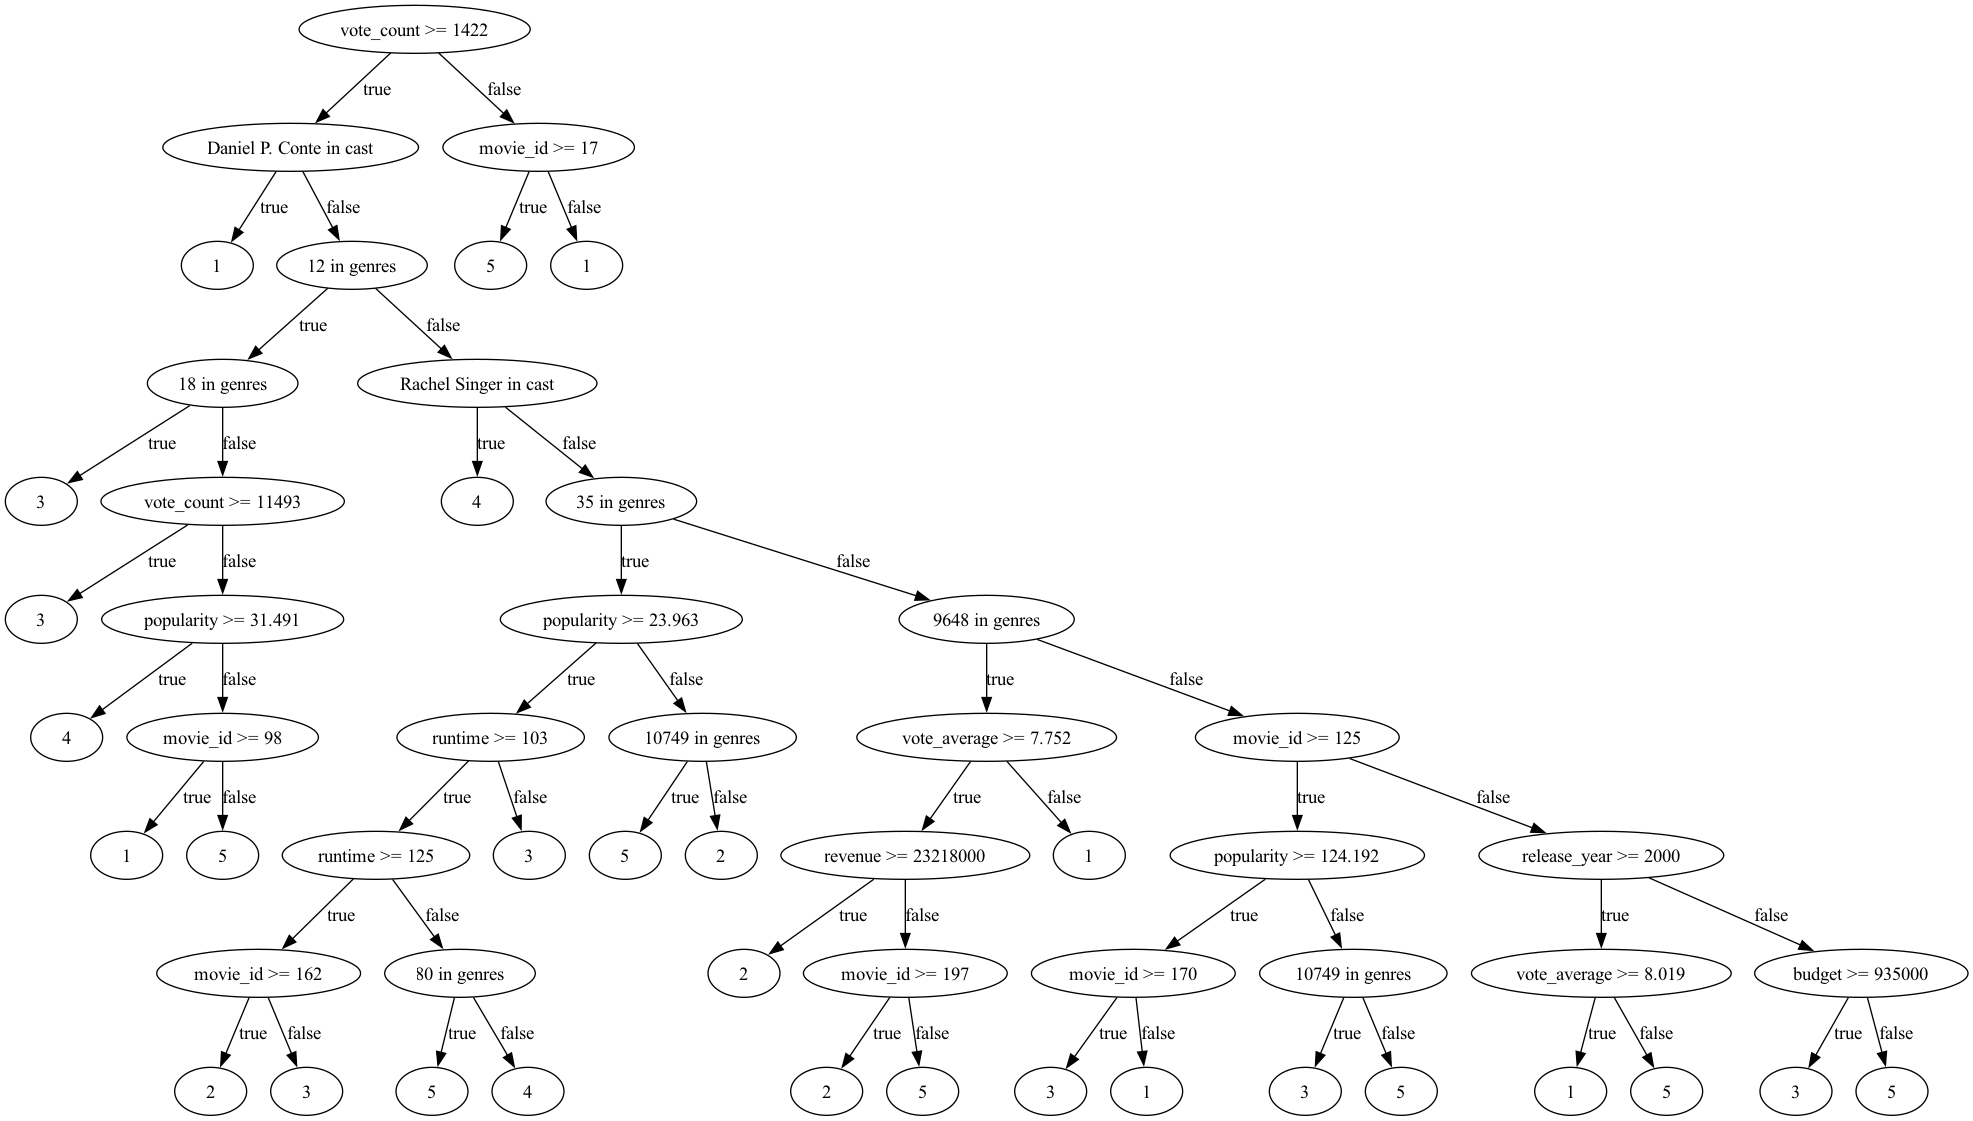
\includegraphics[width=0.4\textwidth]{tree}
    \caption{Visualization of an induced decision tree for a single user.}
    \label{fig:decision_tree}
\end{figure}

\subsection{Results}
The performance metrics indicated:

\begin{table}[h]
    \centering
    \begin{tabular}{|l|c|c|}
        \hline
        \textbf{Metric} & \textbf{Training Data} & \textbf{Validation Data} \\ \hline
        Accuracy        & [add value]         & [add value]           \\ \hline
        Precision       & [add value]         & [add value]           \\ \hline
        Recall          & [add value]         & [add value]           \\ \hline
        Gini Impurity Reduction & [add value]   & [add value]           \\ \hline
    \end{tabular}
    \caption{Metrics on the Training and Validation Datasets}
    \label{tab:performance_metrics}
\end{table}

The decision tree demonstrated its capability to identify patterns in user preferences,
particularly for features such as genre or director, which strongly influenced ratings.
However, its performance was constrained by the simplicity of single decision trees, which tend to make rigid,
binary splits.
The improvement can involve ensemble methods, such as random forests, to enhance generalization,
which is presented in the next section.

\section{Random Forest Approach}
\subsection{Overview}
The Random Forest approach is an ensemble learning method that combines multiple decision trees
to enhance predictive performance and reduce overfitting.
By aggregating the predictions of several individual trees, Random Forest mitigates the limitations of
single decision trees, such as sensitivity to noise and high variance.
To train the Random Forest model, features extracted from the TMDB dataset were used, including \texttt{director},
\texttt{genres}, \texttt{runtime}, \texttt{popularity}, and other attributes.
The ensemble's diversity was assured through two key mechanisms: the random selection of feature
subsets for each tree and the use of bootstrapped training datasets, ensuring that each tree received
a unique perspective on the data.

The Random Forest model was implemented with the
following key components:

\begin{itemize}
    \item \textbf{Random Feature Selection}:
    A custom class, \texttt{\_RandomFeatureSelector}, was created to randomly select a subset of features for each tree. This ensured that individual trees focused on different attributes of the data, reducing the correlation between trees in the ensemble. For example, features like \texttt{budget}, \texttt{genres}, and \texttt{popularity} were considered, while identifiers such as \texttt{title} were excluded to enhance generalization.
    \item \textbf{Bootstrapping}:
    To further ensure diversity, bootstrapped training datasets were generated by sampling movies with replacement from the original dataset. Each bootstrapped sample included selected features and their corresponding ratings.
    \item \textbf{Binary Decision Trees}:
    Each decision tree in the Random Forest was built using binary splits, where node conditions were satisfied or not. The maximum tree depth was restricted to 5 to balance computational efficiency and model expressiveness. The trees were trained to optimize the Gini impurity at each split, ensuring effective feature selection during induction.
    \item \textbf{Aggregation of Predictions}:
    The Random Forest model combined the predictions of all trees in the ensemble using an averaging function. This aggregation reduced the variance of individual predictions and improved the robustness of the final recommendation scores.
\end{itemize}

The Random Forest ensemble operates under the following principles to ensure diversity and robustness:

\begin{enumerate}
    \item \textbf{Random Subsets of Features}:
    Each tree is trained on a randomly selected subset of features, ensuring that individual trees specialize in different aspects of the data. This approach decreases the likelihood of overfitting to specific features.
    \item \textbf{Bootstrapped Datasets}:
    Individual trees are trained on datasets created through bootstrapping, where samples are drawn randomly with replacement from the original training data. This process introduces variability and ensures that each tree receives a unique training set.
    \item \textbf{Prediction Aggregation}:
    During inference, the predictions from all individual trees are aggregated using an averaging function. For instance, if the trees predict ratings of \{3, 4, 3, 4, 5\}, the final recommendation score is calculated as their average.
\end{enumerate}

These principles collectively ensure that the Random Forest model reduces overfitting while maintaining high predictive accuracy.

Since decision trees are interpretable models, it is possible to visualize the decision-making process of individual trees within the Random Forest. Figure~\ref{fig:random_forest_trees} illustrates sample decision trees from the ensemble for a single user. Each tree captures a unique hierarchical structure based on feature thresholds, contributing to the ensemble's diversity.

\begin{figure}[h!]
    \centering
    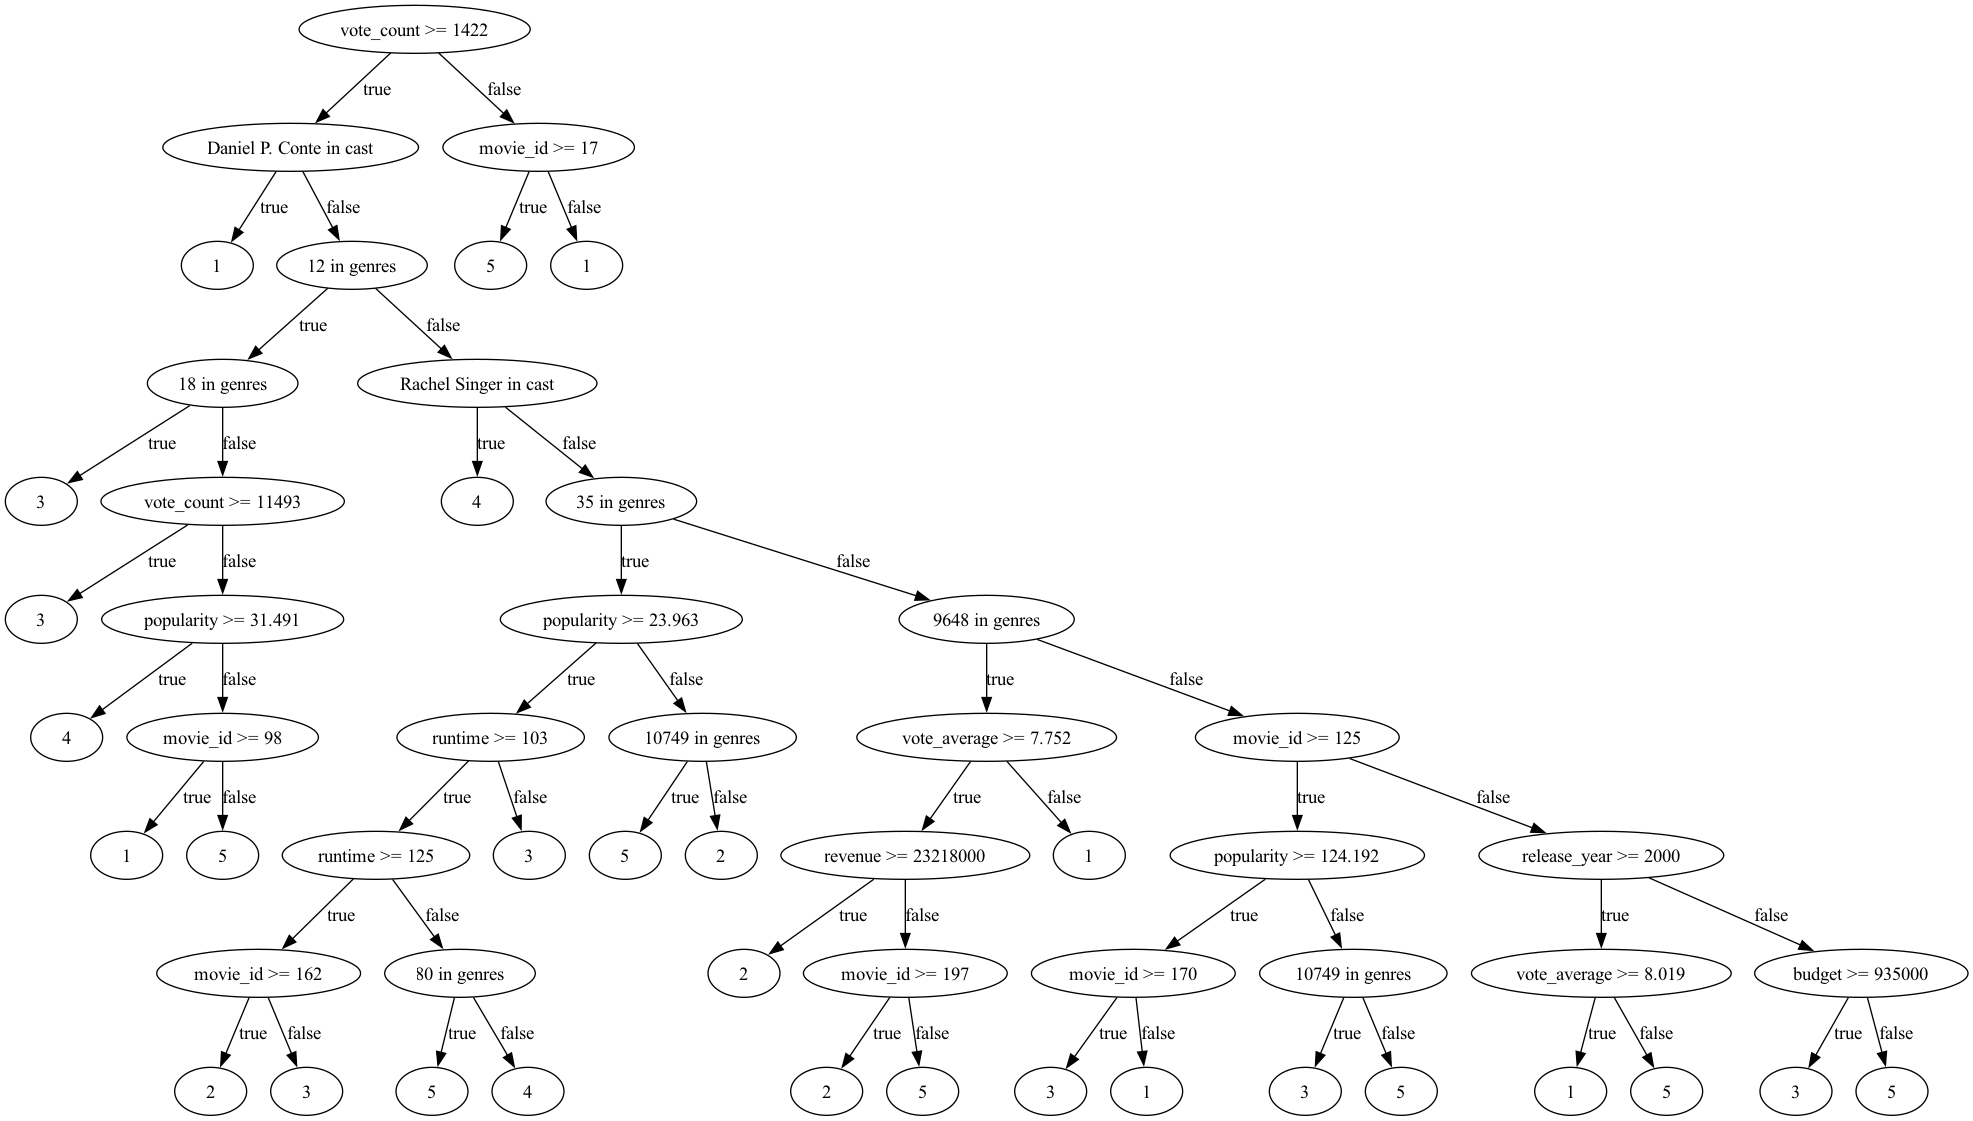
\includegraphics[width=0.4\textwidth]{tree} %TODO: add image
    \caption{Sample decision trees from the Random Forest ensemble for a single user. Each tree reflects a unique subset of features and bootstrapped training data.}
    \label{fig:random_forest_trees}
\end{figure}

\subsection{Results}
The performance metrics indicated:

\begin{table}[h]
    \centering
    \begin{tabular}{|l|c|c|}
        \hline
        \textbf{Metric} & \textbf{Training Data} & \textbf{Validation Data} \\ \hline
        Accuracy        & [add value]         & [add value]           \\ \hline
        Precision       & [add value]         & [add value]           \\ \hline
        Recall          & [add value]         & [add value]           \\ \hline
        Gini Impurity Reduction & [add value]   & [add value]           \\ \hline
    \end{tabular}
    \caption{Metrics on the Training and Validation Datasets}
    \label{tab:performance_metrics}
\end{table}

The results indicate that the Random Forest model significantly outperformed the
single decision tree approach.
By leveraging ensemble diversity, the model effectively captured complex relationships
between features, resulting in improved generalization and predictive performance.

In summary, the Random Forest approach is robust to overfitting,
especially when working with noisy or complex datasets.
Additionally, the embedded feature selection process simplifies model training
by automatically identifying important attributes.

However, despite its strengths, Random Forest models can become computationally expensive for large datasets.
Furthermore, the interpretability of the ensemble is reduced compared to individual decision trees.

\section{Person Similarity Approach}
\subsection{Overview}
The Person Similarity approach was employed to predict user ratings for movies by leveraging the similarity
between users based on their historical ratings.
The primary goal was to identify users with similar movie preferences and use their ratings to estimate
the target user's missing ratings.
This approach exclusively considers user evaluations, disregarding movie-specific features, and focuses
on users who have rated the same movies as the target user.

The methodology for similarity measure involved the combination of \textbf{Pearson correlation} and \textbf{Cosine similarity}:

\begin{itemize}
    \item \textbf{Pearson Correlation:} Captures the linear relationship between two users' ratings, centering around their respective mean ratings to account for rating biases.
    \begin{equation}
        \text{Pearson Similarity} = \frac{\sum_{i} (x_i - \bar{x})(y_i - \bar{y})}{\sqrt{\sum_{i} (x_i - \bar{x})^2 \sum_{i} (y_i - \bar{y})^2}},
    \end{equation}
    where \( x_i \) and \( y_i \) are ratings given by two users for the same movies, and \( \bar{x} \), \( \bar{y} \) are their respective mean ratings.

    \item \textbf{Cosine Similarity:} Evaluates the angular similarity between two users' rating vectors, ignoring the magnitude of their ratings:
    \begin{equation}
        \text{Cosine Similarity} = \frac{\sum_{i} x_i y_i}{\sqrt{\sum_{i} x_i^2} \sqrt{\sum_{i} y_i^2}}.
    \end{equation}
\end{itemize}


A tunable weighting factor, \( \text{pearson\_weight} \), was used to blend the two metrics:
\begin{equation}
    \text{Combined Similarity} = \text{pearson\_weight} \cdot \text{Pearson Similarity} + (1 - \text{pearson\_weight}) \cdot \text{Cosine Similarity}.
\end{equation}
This approach allowed flexibility in prioritizing either metric based on the validation performance.

To mitigate the influence of users with very few overlapping ratings, a damping factor was applied, scaling down the
similarity score when the number of shared ratings was low.

For efficiency, computed similarity scores were cached in a dictionary, avoiding redundant calculations when the same user
pairs were compared multiple times.

To predict the target user's rating for a specific movie, only users who had rated the target movie and shared common
rated movies with the target user were considered for prediction.

The predicted rating, \( \hat{r}_{u,m} \), was calculated using a weighted average of ratings from similar users:
\begin{equation}
    \hat{r}_{u,m} = \frac{\sum_{v \in N(m)} sim(u,v) \cdot r_{v,m}}{\sum_{v \in N(m)} |sim(u,v)|},
\end{equation}
where \( \hat{r}_{u,m} \) is the predicted rating for user \( u \) on movie \( m \), \( sim(u,v) \) is the similarity score between user \( u \) and user \( v \), and \( r_{v,m} \) is the rating given by user \( v \) to movie \( m \). \( N(m) \) denotes the set of users who have rated movie \( m \).

In cases where insufficient overlapping ratings were available, predictions defaulted to the target user's global average rating for better generalization.

\subsection{Results}
The performance metrics indicated:

\begin{table}[h]
    \centering
    \begin{tabular}{|l|c|c|}
        \hline
        \textbf{Metric} & \textbf{Training Data} & \textbf{Validation Data} \\ \hline
        Accuracy        & [add value]         & [add value]           \\ \hline
        Precision       & [add value]         & [add value]           \\ \hline
        Recall          & [add value]         & [add value]           \\ \hline
        Gini Impurity Reduction & [add value]   & [add value]           \\ \hline
    \end{tabular}
    \caption{Metrics on the Training and Validation Datasets}
    \label{tab:performance_metrics}
\end{table}

The Person Similarity approach demonstrated a strong ability to predict user ratings,
particularly in scenarios where users had rated a substantial number of common movies.
However, its performance was more limited when the overlap of rated movies was small, as the approach relies heavily
on the availability of common ratings for comparison.

In conclusion, while the Person Similarity approach provides an effective method for movie rating prediction based on user
similarities, its performance can be impacted by the sparsity of the rating matrix.
Nonetheless, it remains a valuable technique for collaborative filtering in recommender systems.

\section{Collaborative Filtering Approach}
Collaborative filtering is a method used for making automatic predictions about the interests of a user by collecting preferences or taste information from many users. This approach assumes that if a user has agreed with another user on one issue, they are likely to agree on other issues as well.

\subsection{Overview}
This model was trained using a matrix factorization technique, where the user-item interaction matrix (ratings) was decomposed into two lower-dimensional matrices: one representing user parameters and the other representing movie features. This approach allows the model to learn latent factors that explain user preferences and movie characteristics.

\paragraph{Dimensionality Selection}
In our implementation, we initialized the feature space with a dimensionality of 15. This choice was based on empirical testing, balancing model complexity and performance. A higher dimensionality can capture more nuanced patterns but may lead to overfitting. Therefore, we monitored performance metrics on the training set and adjusted dimensionality as necessary to optimize generalization.

\paragraph{Generalization Methods}
To ensure that the model generalizes well to unseen data, several techniques were employed:

\begin{itemize}
    \item \textbf{Regularization}: Both the user and movie feature matrices were subjected to regularization to prevent overfitting. The regularization parameter is denoted as \( \lambda \), and it is applied as follows:
    \begin{equation}
        L = \sum_{u=1}^{U} \sum_{m=1}^{M} \left( \hat{y}(m,u) - y(m,u) \right)^2 + \lambda \left( \|P\|^2 + \|X\|^2 \right) \tag{1}
    \end{equation}
    where \(P\) and \(X\) represent the user and movie feature matrices, respectively.

    \item \textbf{Mean Normalization}: Prior to training, mean normalization was applied to the ratings. This involves centering the ratings around zero:
    \begin{equation}
        \bar{y}_m = \frac{1}{U} \sum_{u=1}^{U} y(m,u) \tag{2}
    \end{equation}
    The normalized ratings are given by:
    \begin{equation}
        y'_{m,u} = y_{m,u} - \bar{y}_m \tag{3}
    \end{equation}

    \item \textbf{Validation and Cross-Validation}: To assess the model’s generalization abilities, we employed \( k \)-fold cross-validation (with \( k = 5 \)). The process involves splitting the dataset into \( k \) subsets and iteratively training and validating the model on different combinations of these subsets.
\end{itemize}

\paragraph{Algorithm Implementation}
Our implementation details for the collaborative filtering model are as follows:

\subparagraph{Movie Ratings}
Let \( y_{m,u} \), or alternatively \( y[m,u] \), denote the rating of movie \( m \) by user \( u \). Therefore, \( y \) will be an \( M \times U \) matrix:
\begin{equation}
y =
\begin{bmatrix}
y_{1,1} & y_{1,2} & \cdots & y_{1,U} \\
y_{2,1} & y_{2,2} & \cdots & y_{2,U} \\
\vdots & \vdots & \ddots & \vdots \\
y_{M,1} & y_{M,2} & \cdots & y_{M,U}
\end{bmatrix} \tag{4}
\end{equation}
Valid ratings are integers from 0 to 5. If \( y_{m,u} \) takes the value of NaN, it denotes that user \( u \) did not rate movie \( m \).

\subparagraph{Movie Features}
Let \( N \) be the total number of features. Then, \( x_{m,n} \) will be the \( n \)-th feature of the movie \( m \). As such, \( x \) will be an \( M \times N \) matrix:
\begin{equation}
x =
\begin{bmatrix}
x_{1,1} & x_{1,2} & \cdots & x_{1,N} \\
x_{2,1} & x_{2,2} & \cdots & x_{2,N} \\
\vdots & \vdots & \ddots & \vdots \\
x_{M,1} & x_{M,2} & \cdots & x_{M,N}
\end{bmatrix} \tag{5}
\end{equation}

\subparagraph{User Parameters}
Each user \( u \) will have a set of parameters \( p_u \) corresponding to the movie features, plus one additional feature \( p_{u,0} \):
\begin{equation}
p =
\begin{bmatrix}
p_{1,0} & p_{1,1} & p_{1,2} & \cdots & p_{1,N} \\
p_{2,0} & p_{2,1} & p_{2,2} & \cdots & p_{2,N} \\
\vdots & \vdots & \vdots & \ddots & \vdots \\
p_{U,0} & p_{U,1} & p_{U,2} & \cdots & p_{U,N}
\end{bmatrix} \tag{6}
\end{equation}

\paragraph{Calculating Predictions}
The predicted rating of movie \( m \) by user \( u \) will be denoted as \( \hat{y}(m,u) \). It will be calculated as follows:
\begin{equation}
\hat{y}(m,u) = p_{u,0} + \sum_{n=1}^N p_{u,n} \cdot x_{m,n} \tag{7}
\end{equation}
Alternatively, as a dot product:
\begin{equation}
\hat{y}(m,u) = p_{u,0} + p[u,1:] \cdot x[m,:] \tag{8}
\end{equation}
where
\begin{equation}
p[u,1:] = \begin{bmatrix}
p_{u,1} & p_{u,2} & \cdots & p_{u,N}
\end{bmatrix}, \tag{9}
\end{equation}
and
\begin{equation}
x[m,:] = \begin{bmatrix}
x_{m,1} & x_{m,2} & \cdots & x_{m,N}
\end{bmatrix}. \tag{10}
\end{equation}

\paragraph{Calculating Errors}
The error function will be as follows:
\begin{equation}
Q(p,x) = \frac{1}{2} \sum_{m,u : y[m,u] \neq -1} (\hat{y}(m,u) - y[m,u])^2 \tag{11}
\end{equation}

\paragraph{Partial Derivatives}
\subparagraph{Zeroth User Parameter}
\begin{equation}
\frac{\partial Q}{\partial p_{u,0}} = \sum_{m : y[m,u] \neq -1} (\hat{y}[m,u] - y[m,u]) \tag{12}
\end{equation}

\subparagraph{Other User Parameters (\(1, \ldots, N\))}
\begin{equation}
\frac{\partial Q}{\partial p_{u,n}} = \sum_{m : y[m,u] \neq -1} (\hat{y}[m,u] - y[m,u]) \cdot x[m,n] \tag{13}
\end{equation}

\subparagraph{Movie Parameters}
\begin{equation}
\frac{\partial Q}{\partial x_{m,n}} = \sum_{u : y[m,u] \neq -1} (\hat{y}[m,u] - y[m,u]) \cdot p[u,n] \tag{14}
\end{equation}

The collaborative filtering approach demonstrated promising results in predicting user ratings for movies. The training process involved iterating over multiple epochs and adjusting the parameters based on the computed gradients. The loss function focused on minimizing the difference between predicted and actual ratings, defined as:
\begin{equation}
Q(P, X) = \frac{1}{2} \sum_{m,u : y(m,u) \neq \text{NaN}} \left( \hat{y}(m,u) - y(m,u) \right)^2 \tag{15}
\end{equation}
\subsection{Results}
The training phase achieved a stable loss value after multiple iterations.
The following metrics were used to evaluate performance:

\begin{table}[h]
    \centering
    \begin{tabular}{|l|c|c|}
        \hline
        \textbf{Metric} & \textbf{Training Data} & \textbf{Validation Data} \\ \hline
        Correct Predictions & [add value]         & [add value]           \\ \hline
        One-Off Predictions & [add value]         & [add value]           \\ \hline
    \end{tabular}
    \caption{Performance Metrics on Training and Validation Datasets}
    \label{tab:predictions_metrics}
\end{table}

The model was validated on a separate dataset to assess its ability to generalize.
Cross-validation techniques (e.g., \(k\)-fold cross-validation with \(k=5\)) were employed to mitigate variance due to data partitioning.
These results demonstrate the effectiveness of the collaborative filtering approach, with a balance between
fitting the training data and generalizing to unseen data.

\section{Summary and Comparison}
- Summarize the results for all approaches using test data or feedback.
- Compare performance metrics and discuss the strengths and weaknesses of each method.
- [Include a table or graph for comparison, if applicable].

\section*{References}
[List any references or sources used in the preparation of the report].

\end{document}